\documentclass{article}\usepackage[]{graphicx}\usepackage[]{color}

\usepackage{alltt}
\usepackage{float}
\usepackage{graphicx}
\usepackage{tabularx}
\usepackage{siunitx}
\usepackage{amssymb} % for math symbols
\usepackage{amsmath} % for aligning equations
\usepackage{textcomp}
\usepackage{booktabs}
\usepackage{mdframed}
\usepackage{natbib}
\usepackage{comment}
\usepackage{booktabs}
\usepackage[colorinlistoftodos]{todonotes} % to make comments on the margin
\usepackage[small]{caption}
\setlength{\captionmargin}{30pt}
\setlength{\abovecaptionskip}{0pt}
\setlength{\belowcaptionskip}{10pt}
\topmargin -1.5cm        
\oddsidemargin -0.04cm   
\evensidemargin -0.04cm
\textwidth 16.59cm
\textheight 21.94cm 
%\pagestyle{empty} %comment if want page numbers
\parskip 7.2pt
\renewcommand{\baselinestretch}{1.5}
\parindent 0pt
%\usepackage{lineno}
%\linenumbers

%% R Script

\title{Unravelling the phenology-phylogeny tangle.}

% alternative titles:
%% An expanded bayesian phylogenetic mixed model to unravel the phenology-phylogeny tangle. %% this sounds too methodsy

\begin{document}

\maketitle

\noindent Authors:\\
The Wolkovich Lab in 2019 \& collaborators $^{1,2,3,4}$ % Will Pearse, Jonathan Davies also
\vspace{2ex}\\
\emph{Author affiliations:}\\
$^{1}$Forest \& Conservation Sciences, Faculty of Forestry, University of British Columbia, 2424 Main Mall, Vancouver, BC V6T 1Z4;\\
$^{2}$Arnold Arboretum of Harvard University, 1300 Centre Street, Boston, Massachusetts, USA;\\
$^{3}$Organismic \& Evolutionary Biology, Harvard University, 26 Oxford Street, Cambridge, Massachusetts, USA;\\
$^{4}$Edificio Ciencias, Campus Universitario 28805 Alcalá de Henares, Madrid, Spain\\
 

\vspace{2ex}
$^*$Corresponding author: ignacio.moralesc@uah.es\\
\renewcommand{\thetable}{\arabic{table}}
\renewcommand{\thefigure}{\arabic{figure}}
\renewcommand{\labelitemi}{$-$}
\setkeys{Gin}{width=0.8\textwidth}

%%%%%%%%%%%%%%%%%%%%%%%%%%%%%%%%%%%%%%%%%%%%%%%
%%%%%%%%%%%%%%%%%%%%%%%%%%%%%%%%%%%%%%%%%%%%%%%
\clearpage

\section*{Abstract}

Plants have evolved responses to environmental cues able to inform them about the temporal distribution of key resources---i.e. energy and light. The responses to individual cues such as forcing (or spring warming) have shown to be subjected to some degree of evolutionary conservatism. Yet, plants do not respond to isolated cues but to a combination of interacting cues, which difficults accurate predictions of phenology in the face of environmental change. Whether and how evolution has constrained phenological responses to combinations of interacting cues is not yet understood even when this knowledge could enhance model predictions and inform how different plant lineages have adapted to environmental change along their evolutionary histories. Here we use Bayesian hierarchical models and the most complete dataset on tree species phenological responses measured in experimental conditions to: (a) test if phenological responses to three major interacting cues are conserved phylogenetically when considered jointly, (b) compare the phylogenetic signal in the responses to different cues and, (c) test whether coefficient estimates differ between models assuming phylogenetic independence among species and models that explicitly incorporate phylogeny. Results show non-random phylogenetic structuring of phenological responses, highly variable across species and cues. More interestingly, regression coefficients shift when models control for phylogenetic effects, particularly so for forcing, which becomes the most important cue. Taken together, our results suggest that phylogeny should be incorporated into studies modelling multi-species phenological responses, as such responses have been jointly constrained through evolution and thus are not independent.  

\clearpage


% not yet satisfied about the pitch - this is already said in Davies et al. 2013 
% should we emphasize the fact that we are using experimental/lab data? What are the gains with respect data from the field?

% we need an angle of at least some novelty

%%%%%%%%%%%%%%%%%%%%%%%%%%%%%%%
% Introduction
%%%%%%%%%%%%%%%%%%%%%%%%%%%%%%%
% Meeting call notes: https://github.com/lizzieinvancouver/ospree/wiki/Phylogeny-and-phenology


\section*{Introduction}
Predicting species responses to recent anthropogenic climate change presents a major challenge to ecological forecasting. With rising global temperatures species have shifted northward in space and earlier in time on average, but with high variability \citep{IPCC:2014sm}. Some of this variability is due to the complexity of climate change itself, including regional and seasonal variation in warming that underlies average trends alongside shifts in other climate axes (e.g. precipitation). Much of it, however, is driven by species-specific variation, reflecting evolved differences in species' sensitivities to underlying cues and their interactions, which we know well for only a few well-studied species. Improving forecasts, thus, will require models that allow for species-level differences in responses to complex environmental cues, and a better understanding of the evolutionary constraints that might limit future adaptation to change. % Understanding how different species lineages have evolved their phenotypic responses to the combined effects of environmental change would greatly aid prediction

Decades of research have informed our understanding of how species use environmental cues to time their phenotypic responses with the temporal distribution of key resources and to avoid periods of high abiotic or biotic stress \citep{larcher1980,bonamour2019}. Commonly, however, responses to environmental cues, and their evolution, are studied individually, for example, linking a given phenotypic response to a single cue, such as time of leafout and summed heat during early spring \citep[e.g.,][]{davies2013phylogenetic}. Such efforts ignore a more likely scenario for most phenotypic traits where multiple cues interacting along evolutionary history have shaped responses \citep{Ackerly:2009ly}. For example, species-level growth rates or plant height may be determined by the interaction among several cues---e.g. soil nutrients, water availability and light \citep{larcher1980}. Similarly, many plant and insect species phenolological events are determined by a combination of temperature and light \citep{chuinearees}, and it is likely that additional cues (such as soil moisture) and species physiology, further mediate species responses, but are often less well understood \citep{chuinearees}.

% Given our relatively advanced understanding of the cues driving spring plant phenology is likely an area where we should be able to develop mechanistic models across species ...
Spring plant phenology may represent our best opportunity to improve forecasts of species’ responses to interacting environmental cues. Beyond being the most studied biological impact of climate change, the primary interacting cue system is well established \citep{chuinearees}, especially for temperate woody species where phenology is generally thought to be determined by two components of temperature---chilling (cool temperatures during dormancy period over winter) and forcing (warm temperatures, generally in the spring)---and photoperiod \citep{XXX}. Plant phenology is also one of few phenotypic traits with extensive experimental data on responses to multiple environmental cues across species. Recent multi-species analyses considering forcing, chilling and photoperiod have shown that chilling and forcing together often determine complex non-linear responses to warming \citep{flynn2018,ettinger2020}. These studies have also found remarkable variation across species in their sensitivities to cues, aligning with long-term observational data across thousands of species \citep{XXX}, and suggesting that current models fail to capture the complexity of species-specific responses. 

Research using long-term observational data has highlighted the role that evolutionary history may play in structuring plant phenological responses. Multiple studies have found dates of budburst, leafout and first flowering appear phylogentically conserved and are thus more similar among closely related species \citep{kochmer1986constraints,willis2008phylogenetic,davies2013phylogenetic}. Phylogenetic signal in plant phenology suggests species respones to cues have diverged over macro-evolutionary timescales, helping explain species present day differences. Almost all these studies, however, have focused on the phenotype (e.g., day of year of a phenological event), which is strongly determined by the local environment (e.g., the climate where phenology was measured), rather than species' intrinsic responses to the environment. More direct measures of species repsones may derived from studies examining species long-term change over time [e.g.,][]\citep{willis2008phylogenetic}---likely capturing a composite of multiple cues---or change per $\degree$C \citep{XXXX}---argued to be a proxy for forcing---and similar metrics, instead of day of year \citep[e.g.,][]{CaraDonna2015}. However, approaches using traditional phylogenetic comparative methods \citep{XXXX}% which studies/approaches are these?
, have produced conflicting results. Evidence for phylogenetic conservatism appears to depend on method and species, even varying from one site to the next for the same clade \citep[e.g.,][]{rafferty2017global}, which violates the fundamental idea of shared evolutionary history---the common ancestor of two sets of species cannot pocesses two separate evolutionary histories for the same trait.

If closely related species express similar phenology when exposd to shared environmental cues it could facilitate forecasting to unmeasured species, and provide insights into the evolutionary histories of species sensitivities to different cues, but it will require approaches that better model the evolution of species respones, especially when underlying cues are complex and interacting. Our understanding of the underlying cues that drive spring phenology suggest we need to model phenology as a composite outcome of the underlying cues---chilling, forcing and photoperiod, allowing evolution in the responses to each. By allowing non-stationarity in species responses across phylogeny \citep{davies2019phylogenetically}, such an approach would depart from most previous work and assumptions of traditional phylogenetic comparative methods [e.g. ][] (cite XXX PGLS/PGLMM/MCMCGLMM?), and moves us towards better integrating evolutionary history in models of phenological responses to environmental change.  

Here we present a novel Bayesian framework that extends upon phylogenetic mixed models to examine how chilling, forcing (metrics of temperature) and photoperiod together determine plant phenology. We illustrate our method with an unprecedented dataset on phenological responses to environmental cues determined experimentally for 192 deciduous woody species \cite[by far the most studied group of species in phenology experiments, see][]{ettinger2020}. Our method allows us to ask: which cue has the largest effect on budburst, how do cues vary across species, and how evolutionary history has shaped species responses to individual cues? Our results allow us to identify historical regime shifts (cite Uyeda, Josef C., et al. The evolution of energetic scaling across the vertebrate tree of life) in phenological responses across the plant phylogeny, and have relevenace for forecasting under ongoing change.



\clearpage

%%%%%%%%%%%%%%%%%%%%%%%%%%%%%%%
% Methods
%%%%%%%%%%%%%%%%%%%%%%%%%%%%%%%

\section*{Methods}

Chunks to maybe work in... 
\begin{itemize}
\item Common phylogenetic regression accounts for phylogenetic relationships as a grouping factor either explicitly (PMM) or implicitly (PGLS). Here we present one possible approach that accounts for more complex interactions going on among predictors, which would be reflected in the species-level slopes being allowed to vary as a function of the phylogeny, rather than keeping slopes constant and only allowing the intercepts (or residuals) to vary. 
\item In a first attempt at establishing whether or not it is important, we compare results from a common hierarchical model with partial pooling on the slopes that does not allow for phylogenetic constraints to affect slope estimates against results from a phylogenetic hierarchical model allowing phylogeny to constrain partially pooled slopes. 
\end{itemize}

% Used phylogenetic regression either hierarchical (PMM) or not (PGLS), where only phylogenetic signal or effects are modelled for the residuals (or included as a grouping or random factor). 
\subsection*{Phenological and Phylogenetic Data}
% See _README_paperresearchmethods.txt
\emph{Phenological data:} To estimate phenological responses to chilling, forcing and photoperiod we used data from phenological experiments of temperate woody species conducted in controlled environments, brought together in the Observed Spring Phenology Responses in Experimental Environments (OSPREE) database. In July 2019, we updated an earlier version of this database \citep{wolkovich2019} by reviewing all papers found through searching ISI Web of Science and Google Scholar with the following terms: 
\begin{enumerate}
\item TOPIC = (budburst OR leaf-out) AND (photoperiod OR daylength) AND temperature*, which yielded 623 publications
\item TOPIC = (budburst OR leaf-out) AND dorman*, which yielded 270 publications
\end{enumerate}
We scraped data from all papers of woody species that tested for photoperiod and/or temperature effects on budburst, leafout, or flowering, resulting in 56 papers. \citet{ospreebbms} used a portion (72 experiments across 49 papers) of the earlier OSPREE database and provides extensive methods on the database creation and cleaning. For our analysis here, we included all budburst experiments where we could quantify chilling, forcing and photoperiod levels, resulting in 44 studies from 33 papers. 
% Nacho, please:
% XX add length(unique(datasetID)) from an OSPREE clean file (make sure it does not have strawberries). 
% YY add length(unique(paste(datasetID, study)) from datafile you use in the end ... ditto for ZZ
% Also, we need to publish an updated OSPREE dataset on KNB eventually.
Across experiments chilling treatments were often fully or partially applied in the field, thus we estimated field chilling ourselves using daily temperature data from ... [Cat and Nacho -- add here: Be sure to include updated info on our datasets and which chilling metric we used]. \citet{ospreebbms} provides additional details on these calculations (however, to have climate data through all our study years, we used a different climate dataset here for North America).\\ 
% We could probably add species info above? If you want to contrast with bb ms: \citet{ospreebbms} had 39 years, and 203 species
% Lizzie says ... this methods part feels a little short to me, but I think it may be all we need. (Maybe Ailene can eventually take a look to check what might be missing? But I think we can definitely wait for that until we have a full draft.)
% IMC - I may need help from Cat about the latest chilling data sources, the metric and so on. It will be great to have Ailene double-checking this part.
We analyze 2 different subsets of species in the OSPREE database to explore differences across two major groups of taxa, angiosperms and gymnosperms, for which there are markedly different number of species (194 angiosperms vs. 19 gymnosperms), and whose deep evolutionary divergence advises for separate analyses \citep{}.\\
% IMC - I wonder if we should re-analyze data for the exact subset of species in Ettinger et al. 2020NCC. We mentioned doing so at some point but I never did it.
% EMW (19Mar2022):I woudl skip it until reviewers ask or we think we desperately need it. 


\begin{comment}
\begin{enumerate}
\item Description of the OSPREE database (where it comes from, number of species, studies, etc.). % Lizzie started this -- see above

\item We analyze 5 different subsets of species in the OSPREE database to explore differences across taxa (effect of gymnosperms?) and to test to what extent data resolution affects the results:

\begin{enumerate}
\item Species grouped in generic complexes, to ensure enough cross-treatment data, as in Ettinger et al. (under review) (including 52 complexes)[flags.for.mainmodel=T]
\item All species in the main model (including 117 species resulting from )[flags.for.mainmodel=T]
\item All angiosperm species in the main model (including 110 species)[flags.for.mainmodel=T]
\item All species in the latest version of OSPREE (including 231 species resulting from )[flags.for.allsppmodel=T]
\item All angiosperm species in the latest version of OSPREE (including 215 species)[flags.for.allsppmodel=T]
\end{enumerate}
\end{comment}

We used the phylogenetic megatree for seed plant from \citet{smith2018constructing} to extract a subset phylogenetic tree containing only the species in the OSPREE dataset \citep{wolkovich2019}. We pruned the megatree to generate to sub-trees containing only the species in each subset of data. The species that were not present in the megatree were added as polytomies at the generic level (using the function \emph{congeneric.merge}; \citep{pearse2015pez}) with a branch length of zero. Polytomies represent 26.8\% of the full angiosperm dataset. To test for the ability of polytomies to bias our results we run sensitivity analyses excluding these species from models (which lead to 142 angiosperms; see Supporting Information). \\ 


\subsection*{Bayesian hierarchical phylogenetic model}
% PICs are also sort of a regression phylo thing so adjusted below ..
Commonly used phylogenetic regression methods today (e.g., PGLS and PMM) were originally conceived as statistical corrections for phylogenetic non-independence across observations---generally species---thus allowing multi-species studies to meet the assumptions linear regression \citep{freckleton2002phylogenetic}. These corrections incorporated phylogenetic structure in the regression by modifying the residual variance-covariance matrix to substitute off-diagonal elements of zero (the value given the assumption of independence across observations) for shared phylogenetic branch lengths representing pairwise covariances (under phylogenetic non-independece among observations). Off-diagonals were also allowed to include a multiplying parameter---generally referred to as lambda---which is a transformation indicating the amount of phylogenetic relatedness among species (see below). Because the original aim of these methods was to correct for statistical nuance, the underlying assumption of phylogenetic regressions is that phylogenetic relatedness would only affect either model residuals \citep[in PGLS approaches,][]{freckleton2002phylogenetic}, or the model intercepts \citep[e.g., in many PMM approaches,][]{housworth2004phylogenetic}.\\ 
% IMCmar04 - It would be great to have others (Lizzie, Jonathan and/or Will)reviewing this paragraph to double-check it is accurate

Because our aim is to understand how evolution may have imprinted biological responses to multiple interactive cues, our approach expands the above methods by explicitly incorporating phylogenetic structure accross model intercepts and slopes. Doing so allows explicitly estimating the amount of phylogenetic relatedness in species' sensitivities to each cue, when these sensitivities are modelled in a multi-predictor regression setting.  
% IMCmar04 - starting to flesh out this bit. Needs work.
% EMW (13Mar2022): May want to add a supplement explaining how intercepts and residuals are somewhat similar in our model? Especially as you touch on it above. Geoff has some text for this. 

% The following text is copied from Geoff's PMM description:
For each $j$ species, we assumed that data were generated from the following sampling distribution:

\begin{align}
  \label{modely}
  y_j \sim \mathcal{N}(\mu_j, \sigma_e^2)
\end{align}
where
\begin{align}
  \label{modelmu}
  \mu_j = \alpha_j + \beta_{1,j} X_2 + \beta_{2,j} X_2 + \beta_{3,j} X_3
\end{align}

Predictors $X_1$, $X_2$, $X_3$ are standardized forcing, chilling, and photoperiod, and their effects on the phenology of species $j$ are determined by parameters $\beta_{1,j}$, $\beta_{2,j}$, $\beta_{3,j}$, representing species' responses (or sensitivities) to each of the cues. These responses, including the species-specific intercept $\alpha_j$, are elements of the following normal random vectors:
\begin{align}
    \label{phybetas}
  \boldsymbol{\alpha} = \{\alpha_1, \ldots, \alpha_n\}^T & \text{ such that }
  \boldsymbol{\alpha} \sim \mathcal{N}(\mu_{\alpha},\boldsymbol{\Sigma_{\alpha}}) \\
  \boldsymbol{\beta_1} =  \{\beta_{1,1}, \ldots, \beta_{1,n}\}^T & \text{ such that }
  \boldsymbol{\beta_1} \sim \mathcal{N}(\mu_{\beta_1},\boldsymbol{\Sigma_{\beta_1}}) \nonumber \\
  \boldsymbol{\beta_2} =  \{\beta_{2,1}, \ldots, \beta_{2,n}\}^T & \text{ such that }
  \boldsymbol{\beta_2} \sim \mathcal{N}(\mu_{\beta_2},\boldsymbol{\Sigma_{\beta_2}}) \nonumber \\
  \boldsymbol{\beta_3} =  \{\beta_{3,1}, \ldots, \beta_{3,n}\}^T & \text{ such that }
  \boldsymbol{\beta_3} \sim \mathcal{N}(\mu_{\beta_3},\boldsymbol{\Sigma_{\beta_3}}) \nonumber
\end{align}

\noindent where the means of the multivariate normal distributions are root trait values (i.e., values of cue responses prior to evolving across a phylogenetic tree) and $\boldsymbol{\Sigma_i}$ % we need to decide for a nomenclature that is as widespread/easy to understand as possible. Other papers use bold V, or C to refer to the VCV matrix. Any suggestions are welcome
are $n \times n$ phylogenetic variance-covariance matrices of the form: \\ 
\begin{align}
  \label{phymat}
\begin{bmatrix}
  \sigma^2_i & \lambda_i \times \sigma_{i} \times \rho_{12} & \ldots & \lambda_i \times \sigma_{i} \times \rho_{1n} \\
  \lambda_i \times \sigma_i \times \rho_{21} & \sigma^2_i & \ldots & \lambda_i \times \sigma_{i} \times \rho_{2n} \\
  \vdots & \vdots & \ddots & \vdots \\
  \lambda_i \times \sigma_i \times \rho_{n1} & \lambda_i \times \sigma_i \times \rho_{n2} & \ldots & \sigma^2_i \\
\end{bmatrix}
\end{align}

\noindent where $\sigma_i^2$ is the rate of evolution across a tree for trait $i$ (here assumed to be constant along all branches), $\lambda_i$ scales branch lengths and therefore is a measure of the ``phylogenetic signal'' or extent of phylogenetic relatedness on each model parameter (i.e., $\alpha_{j}$, $\beta_{1,j}$, $\beta_{2,j}$, $\beta_{3,j}$), and $\rho_{xy}$ is the phylogenetic correlation between species $x$ and $y$, or the fraction of the tree shared by the two species.

The above specification is equivalent to writing equation \ref{modelmu} in terms of root trait values and residuals, such that:

\begin{align}
  \label{eqfive}
  \mu_j = \mu_\alpha + \mu_{\beta_1} X_1 + \mu_{\beta_2} X_2 + \mu_{\beta_3} X_3 + e_{\alpha_{j}} + e_{\beta_{1,j}} + e_{\beta_{2,j}} + e_{\beta_{3,j}}
\end{align}

\noindent where the residual error terms (e.g., $e_{\alpha_{j}}$) are elements of normal random vectors from multivariate normal distributions centered on $0$ with the same phylogenetic variance-covariance matrices as in equation \ref{phymat}.



% IMC 15mar - somewhere in the methods (I wonder if here) we should mention the sets of analyses that we run:
% angiosperms phylo model, angiosperms lambda0 model, gymno phylo model, gymno lambda0 model,
% in addition I think we may need angiosperms lambda1 model, gymno lambda1 model
% EMW (19Mar2022): Yes! We really need this, I think it will get the methods section back to our biological aims. 

\subsection*{Interpretation of $\lambda_j$ and $\sigma_j^2$ on slopes and intercepts}

% EMW (28Mar2022): I wonder if we want to be careful about when we use phylogenetic signal versus phylogenetic structure? Do they mean the same thing? 
Most current phylogenetic regression approaches aimed at controlling for phylogenetic non-independence of analysis units \citep[i.e. species, see][]{revell2010phylogenetic} assume the $\lambda$ scaling parameter is constant across the full set of predictors in the model. Thus, $\lambda$ is estimated as a single parameter based on one single residual term VCV matrix. While useful for correcting for phylogenetic non-independence this approach does not allow the phylogeny to differntially affect different predictors (i.e. environmental cues in our example, which refer to simply as cues hereafter). In models with multiple cues, species responses to all cues are estimated as similarly phylogenetically structured, but this may not be the case. For example, in a PGLS model with three cues, it would be possible to have a high (i.e. close to 1) value of $\lambda$, due to either a strong phylogenetic signal in the response, but no phylogenetic structuring in the cues, or one or more predictors being strongly phylogenetically structured. In the latter case, phylogenetic structuring of responses to cues could be correlated (i.e., responses to cues evolving in a correlated fashion) or uncorrelated (i.e., independent evolution of responses to cues). Discerning these different situations is not trivial as they would inform whether responses to predictors configure in a structured fashion along the evolutionary process. However, most current approaches act as a black box regarding this information; they simply inform whether or not model residuals are phylogenetically structured (i.e. in PGLS) or the amount of model variance attributable to the phylogeny and independent from other sources of variation (i.e., in PMM, see \cite{housworth2004phylogenetic}).\\

Because we are specifically interested in estimating the phylogenetic structure of each cues, our approach explicitly partitions variance into specific components relative to the model intercept and predictor (cue) slopes (see equation \ref{eqfive}). The multivariate normal distributions of the intercept and slope terms include each a variance term (see equation \ref{phybetas}), modelled with a $\lambda$ scaling parameter. The interpretation of $\lambda$s in our models are analogous to Pagel's \cite{pagel1999inferring} $\lambda$ parameter \citep{housworth2004phylogenetic}, constrained to range from 0 to 1, with values of 0 indicating absence of phylogenetic relatedness, and values of 1 indicating \emph{Brownian Motion} evolution (BM). Estimated $\lambda$s are not fully equivalent to computing phylogenetic signal of the slopes of each cue separately (i.e., fitting a multilevel regression model with species as a grouping factor on intercepts, and subsequently estimating phylogenetic signal for model slopes). Instead, they are a relative metric of phylogenetic relatedness allowing us to compare among responses known to interact with each other and estimated simultaneously. This approach has the further benefit of adjusting our partial pooling (`random effect' of species) based on evolutionary distance, more strongly pooling closely related species, and only weakly pooling distantly related species \citep[see Gaussian process models in][]{BDA}. \\% While most current approaches compute only one $\lambda$, our approach computes four, one independent of the predictors, and one for each predictor.

A traditional interpretation of $\sigma^2$s under Brownian Motion evolution, is an `evolutionary rate’ or phenotypic accummulation over time \citep{revell2008phylogenetic}. In PGLS, $\sigma_\epsilon^2$ is estimated for the model error term, which is distributed as a multivariate normal with VCV matrix given by $\sigma_\epsilon^2$$\boldsymbol{\Sigma_i}$. Here, similar to our approach to $\lambda$, we estimate four $\sigma^2$ values, corresponding to each model parameter. In our particular case (i.e., modelling a phenological response to three environmental cues), $\sigma_\alpha^2$ for the intercept could be interpreted as the phenological variation across species accummulated along evolution independently from the cues. The $\sigma_\beta_1^2$, $\sigma_\beta_2^2$, and $\sigma_\beta_3^2$, corresponding to model slopes, would represent the phylogenetic variance linked to species responses to each of the modelled cues (i.e., forcing, chilling, and photoperiod, respectively). This is, the variability in how species shift their phenology responding to temperature and light, accummulated along the evolutionary process and considered in concert. \\ 



\bibliography{phylorefs}
\bibliographystyle{amnat}

%%%%%%%%%%%%%%%%%%%%%%%%%%%%%%%
% Tables and Figures
%%%%%%%%%%%%%%%%%%%%%%%%%%%%%%%
\section*{Tables and Figures} 


%IMC 22mar - we should decide among one of the next two figures, instead of having separate figures per cues?
% EMW (28Mar2022): I vote for the first one, but both are great!
\begin{figure} [H]
  \begin{center}
  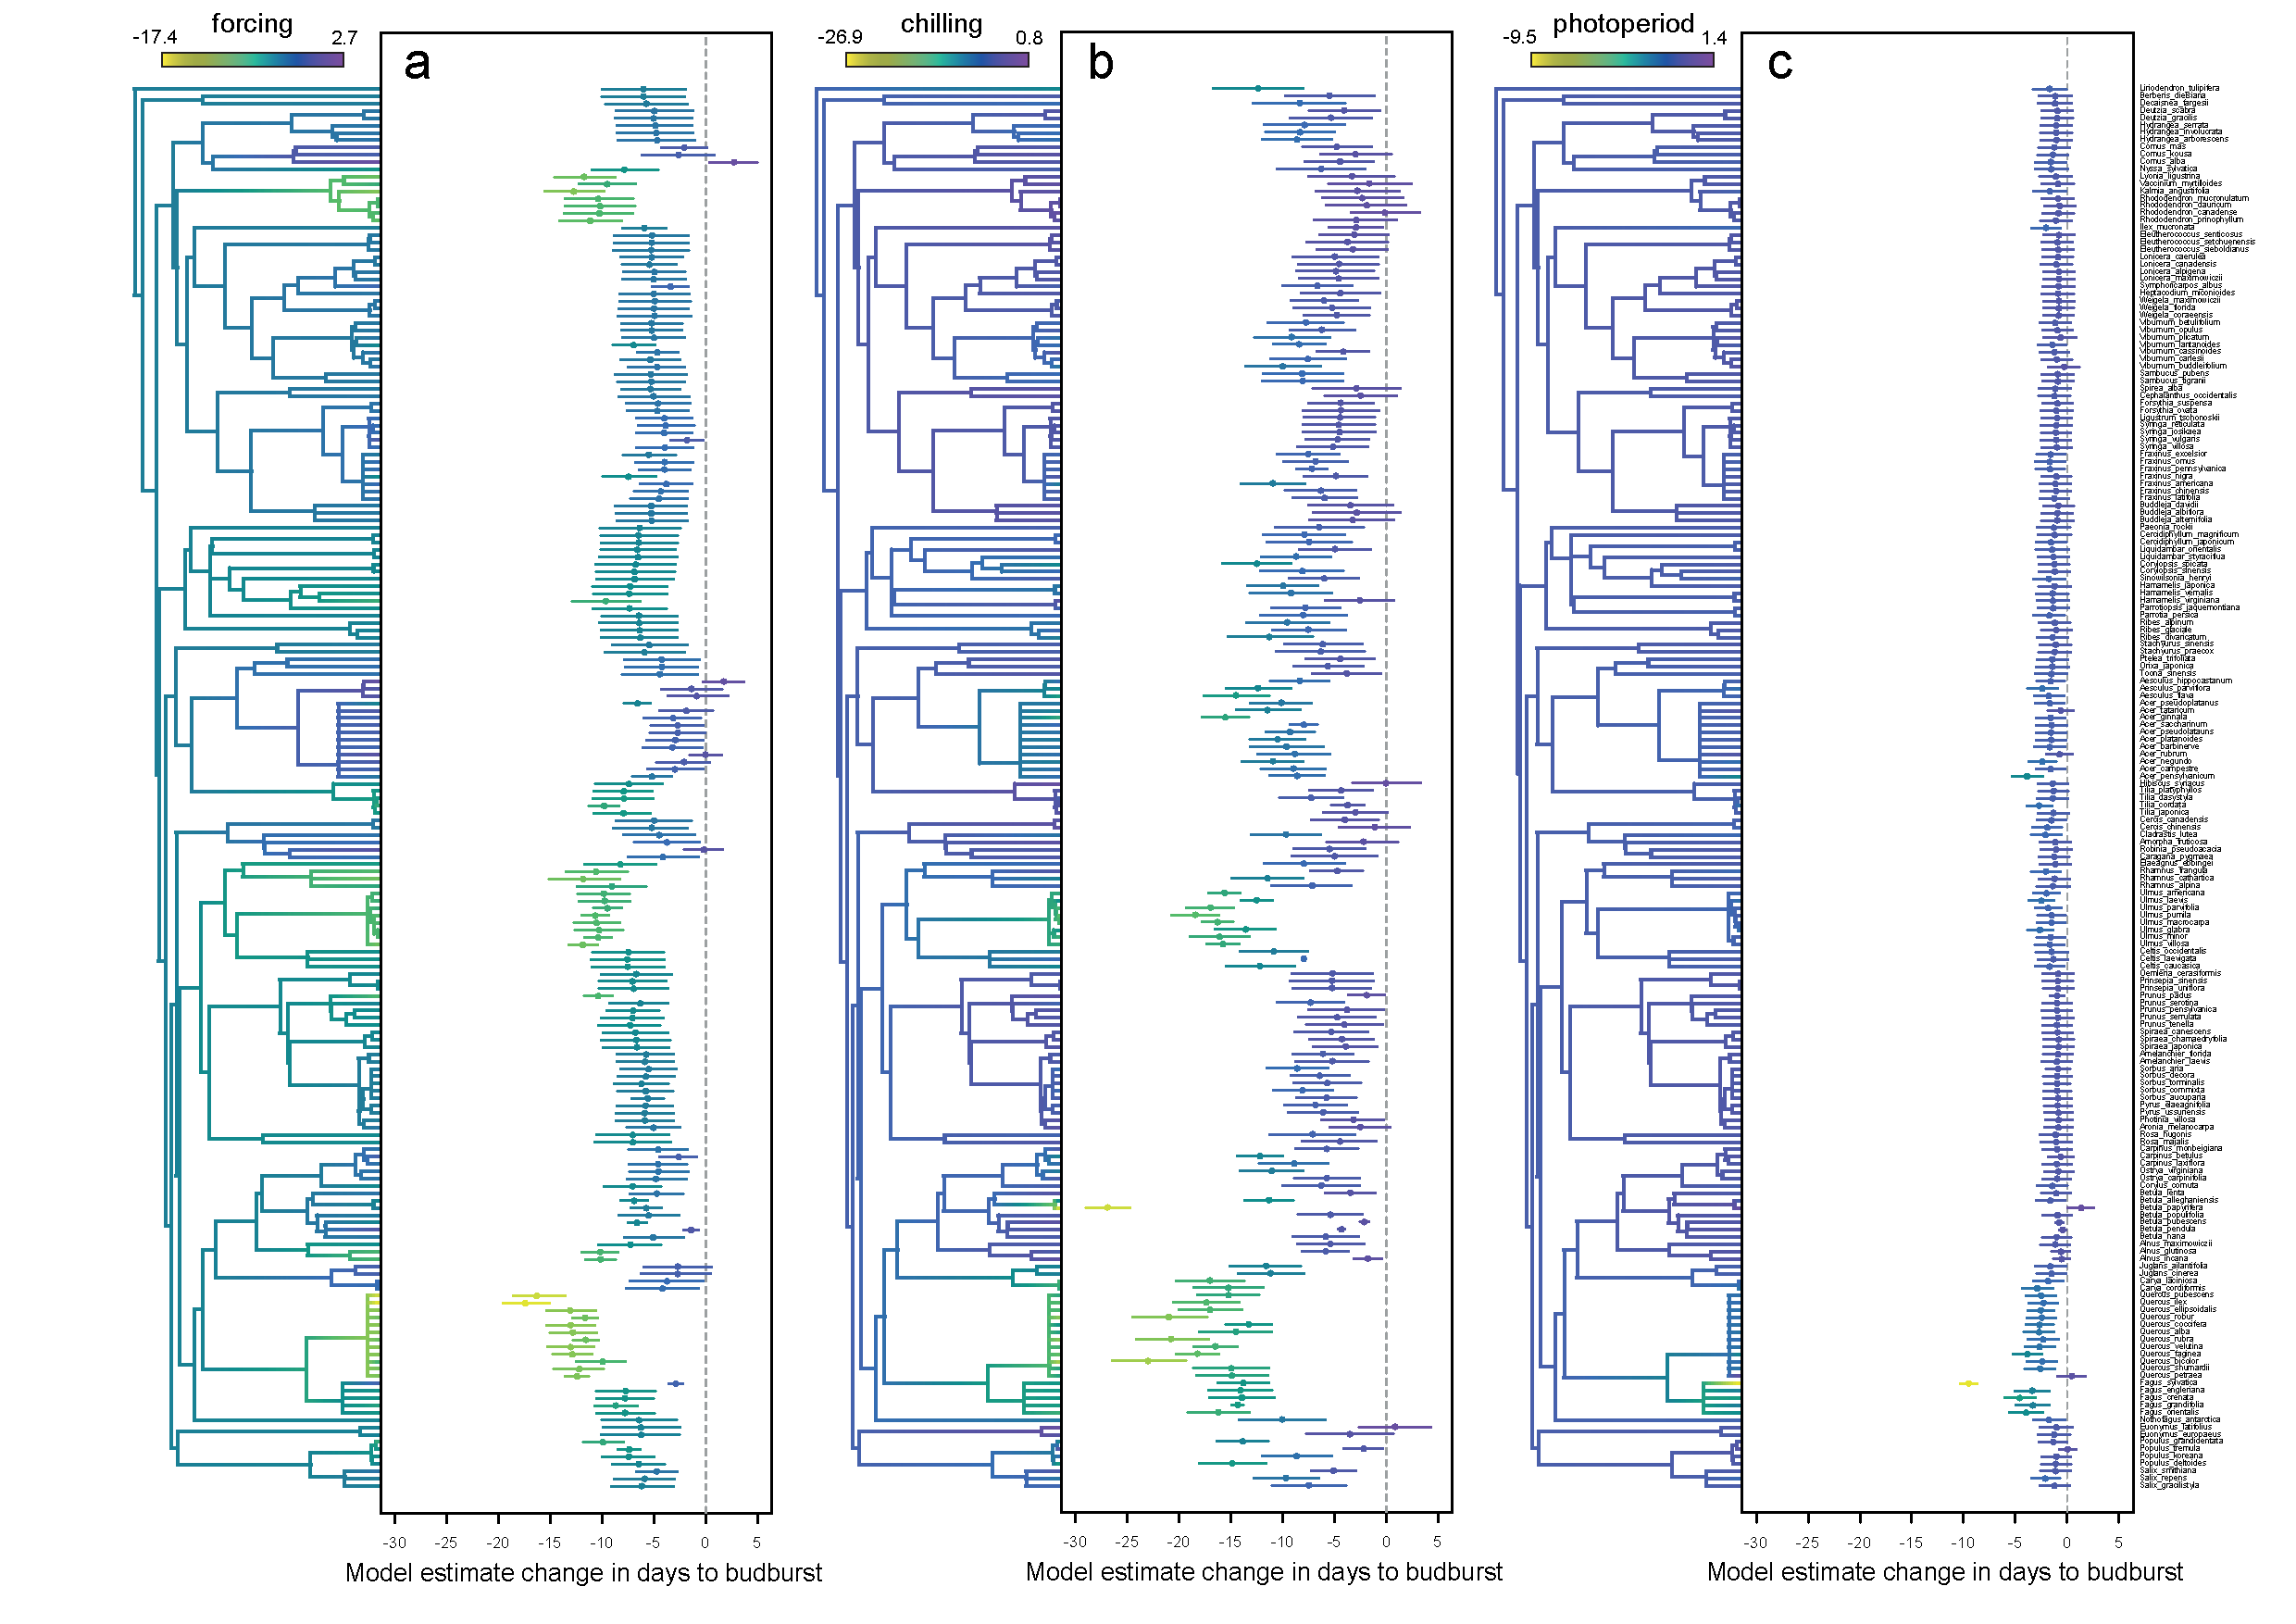
\includegraphics[width=16cm]{../../analyses/phylogeny/figures/muplot_phylo_allcue_angio.pdf}
  \caption{Phenological sensitivity to thee environmental cues, forcing (a), chilling (b) and photoperiod (c) measured in change in days to budburst per standardized unit (z-transformation) of the cues across 192 angiosperm species. The same phylogenetic tree is shown in each panel, colored acording to an estimation of ancestral character states, being the states at the tips the model slopes of our hierarchical phylogenetic model. Note that the color scale varies in each panel. Total tree depth is 81. My.}
  \label{fig:muplot_all}
  \end{center}
\end{figure}

\begin{figure} [H]
  \begin{center}
  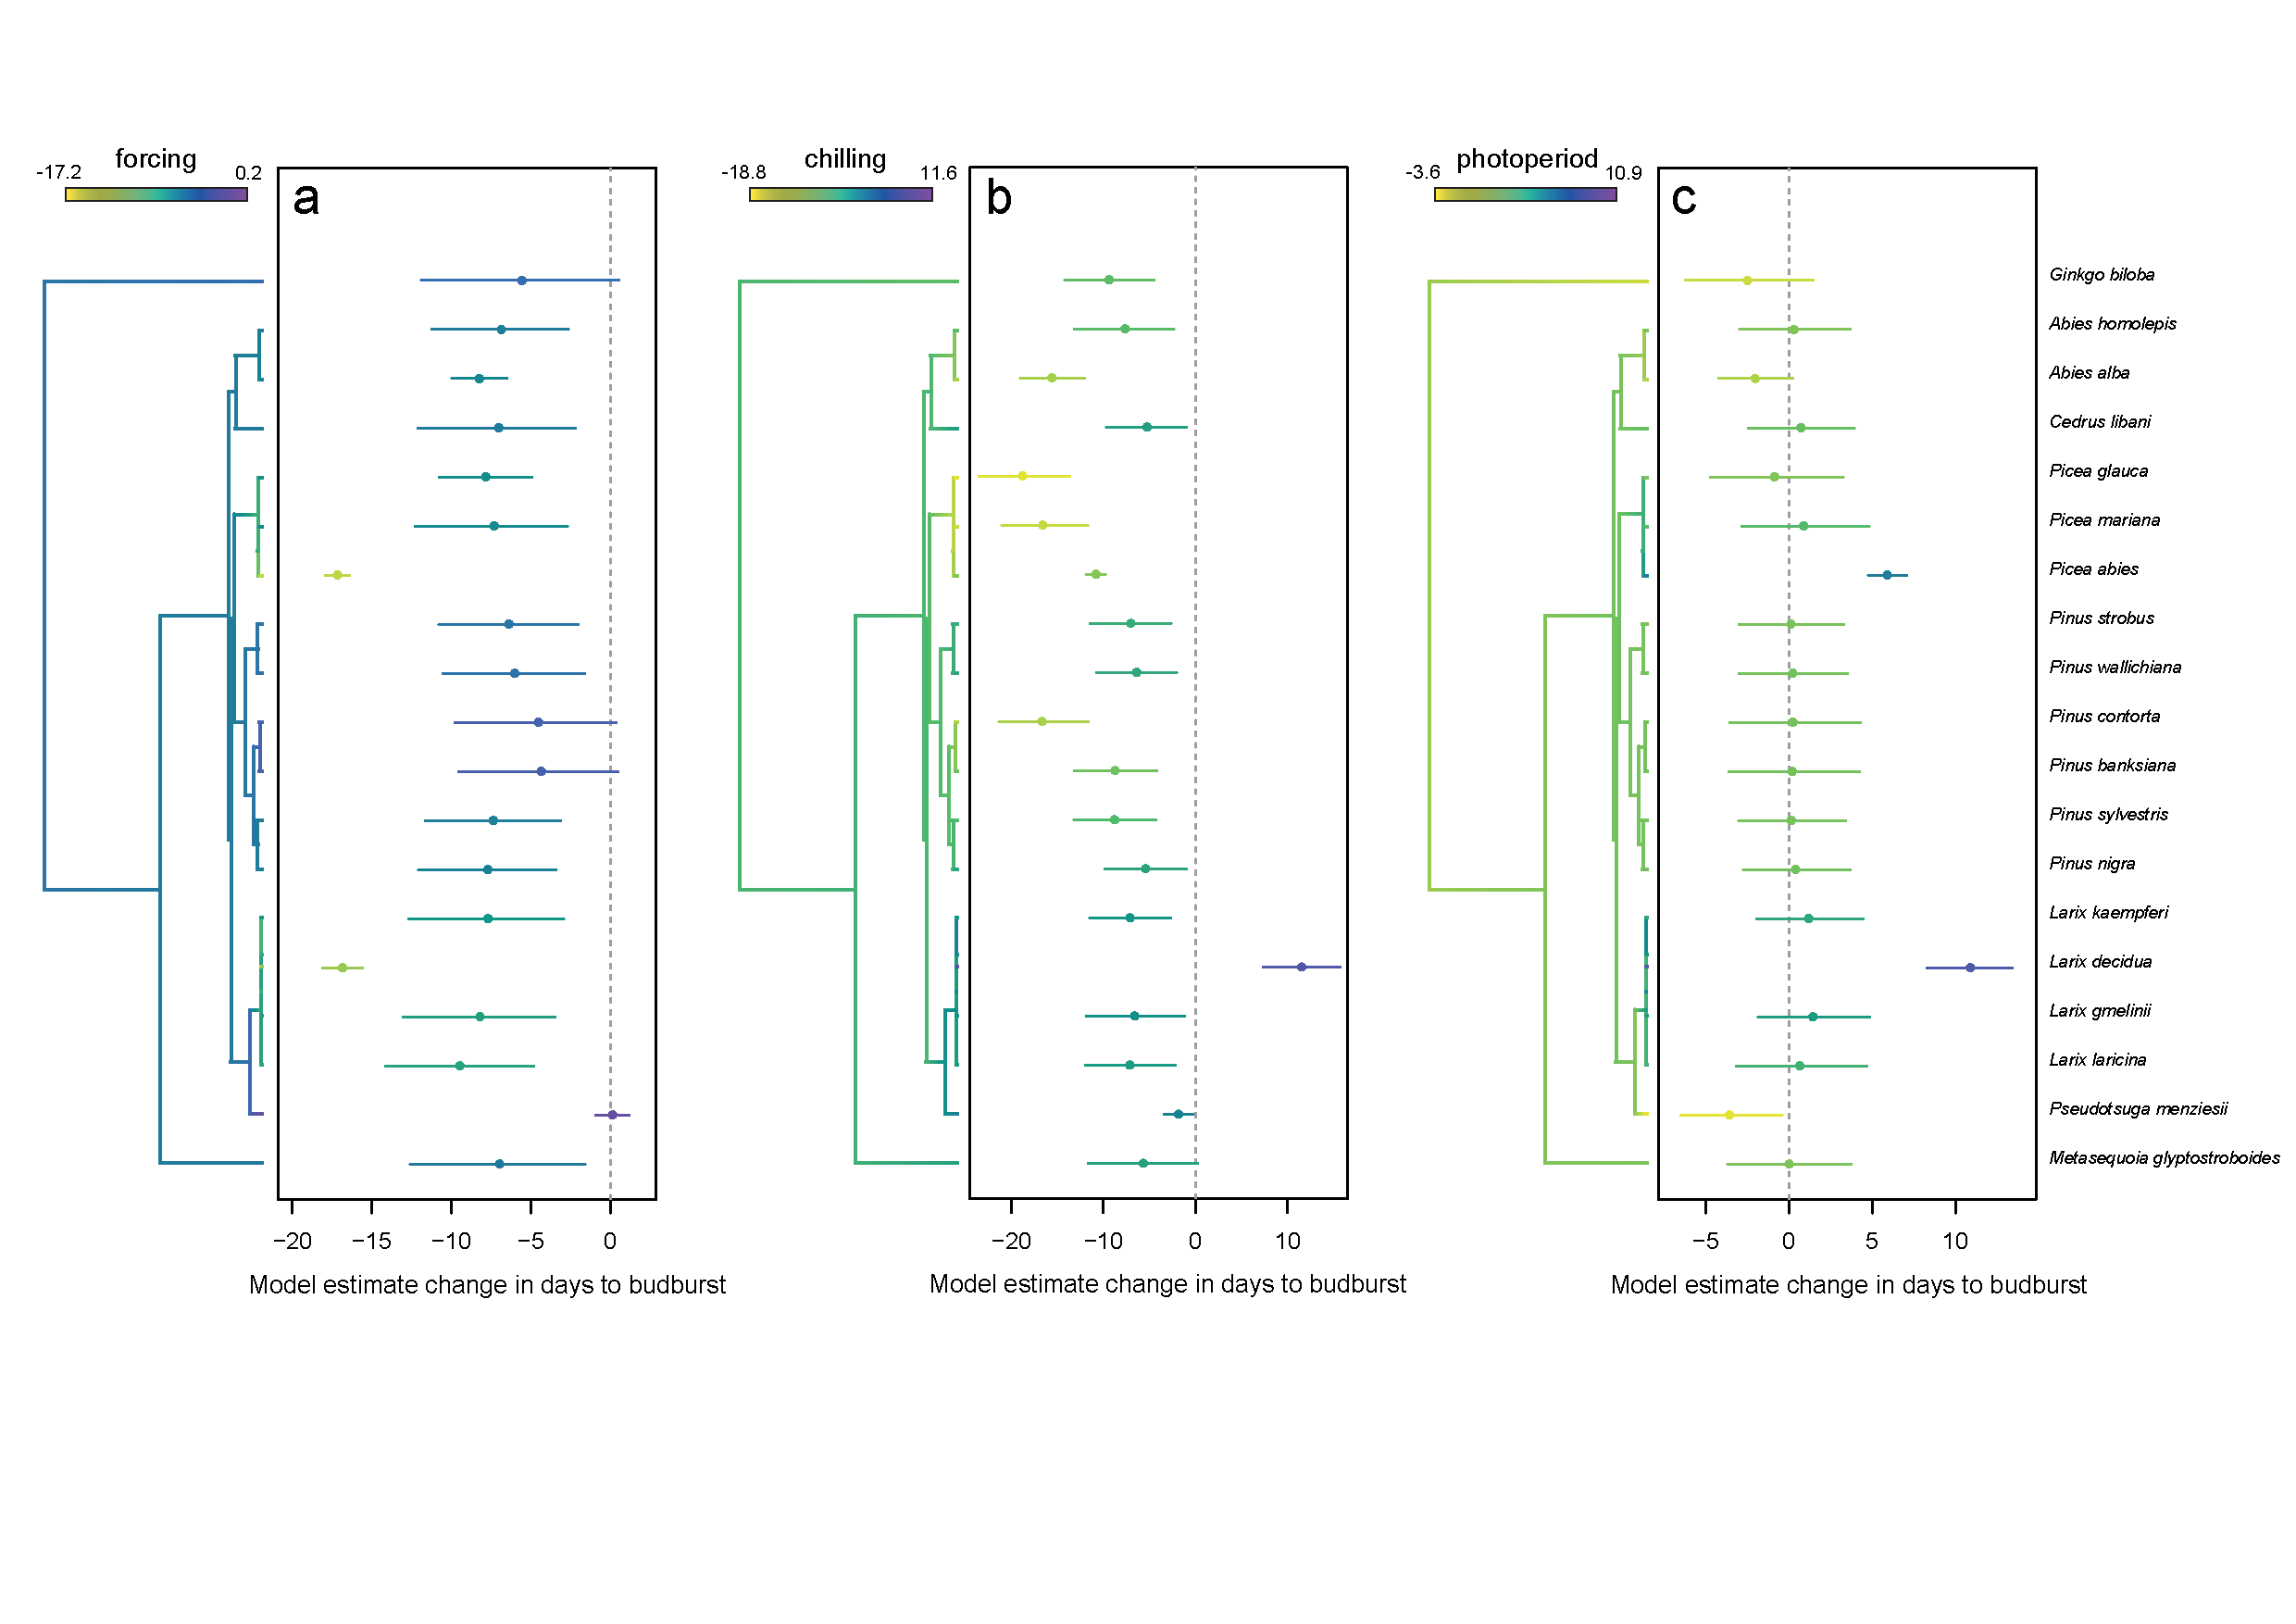
\includegraphics[width=16cm]{../../analyses/phylogeny/figures/Fig1b_phylo_muplots_gymno.pdf}
  \caption{Phenological sensitivity to thee environmental cues, forcing (a), chilling (b) and photoperiod (c) measured in change in days to budburst per standardized unit (z-transformation) of the cues across 19 gymnosperm species. The same phylogenetic tree is shown in each panel, colored acording to an estimation of ancestral character states, being the states at the tips the model slopes of our hierarchical phylogenetic model. Note that the color scale varies in each panel. Total tree depth is 81. My.}
  \label{fig:muplot_allgymno}
  \end{center}
\end{figure}


\begin{figure} [H]
  \begin{center}
  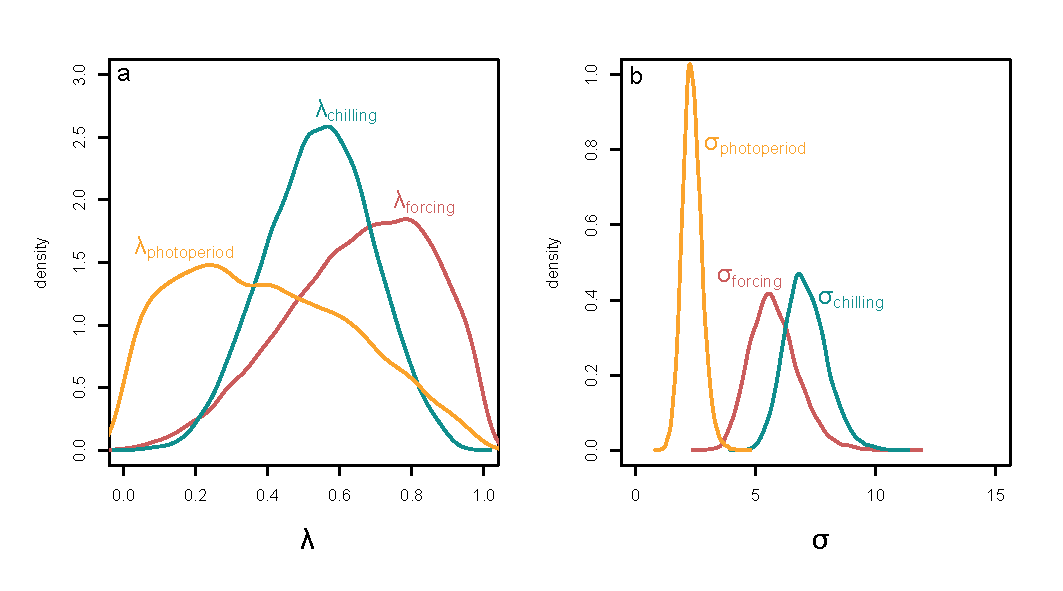
\includegraphics[width=14cm]{../../analyses/phylogeny/figures/Fig2_lambdas_sigmas.pdf}
  \caption{Density plots for the posterior distribution of phylogenetic signal measured by lambda for each cue included as a predictor in the model for angiosperms: forcing (red), chilling (blue),  photoperiod (orange) and for the model intercept (grey). Panels correspond to angiosperms (a-d) and gymnosperms (e-h). Note that lambda estimations corresponding to  panels c-d and g-h as they are constrained to be either equal zero or equal 1.}
  \label{fig:phylosig_all}
  \end{center}
\end{figure}

\begin{figure} [H]
  \begin{center}
  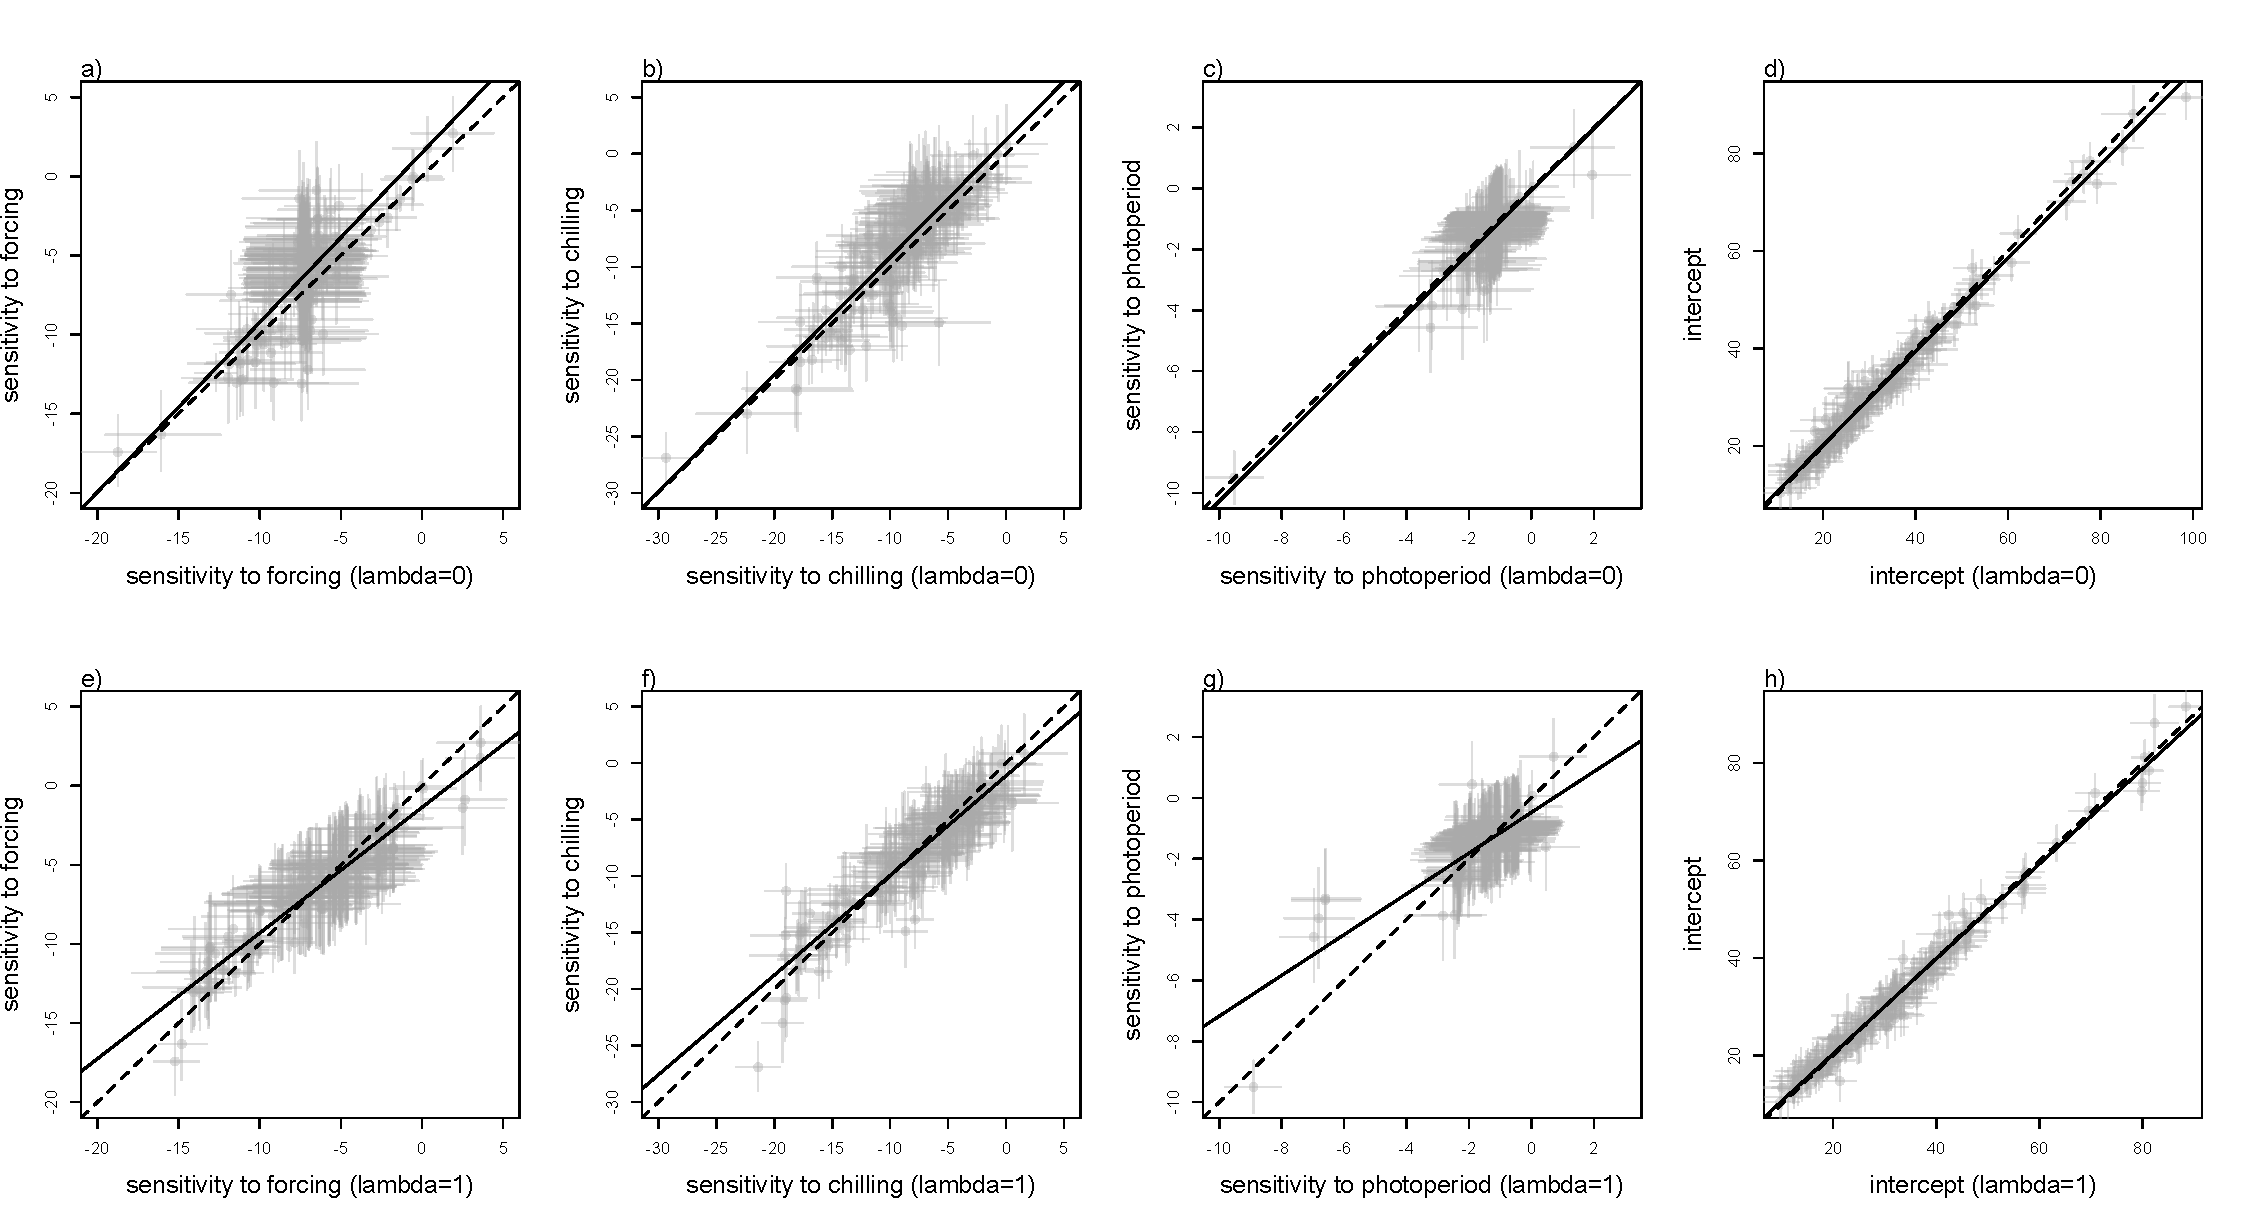
\includegraphics[width=14cm]{../../analyses/phylogeny/figures/Est_correls_vs_lamb01_angio.pdf}
  \caption{Correlations between model parameters as estimated by the full model and the models where lambda is constrained to be equal zero (upper row) or one (bottom row), for angiosperms. Panels correspond to sensitivity to forcing (a,e), to chilling (b,f), to photoperiod (c,g) and to model intercepts (d,h).}
  \label{fig:correls_angio}
  \end{center}
\end{figure}

\begin{figure} [H]
  \begin{center}
  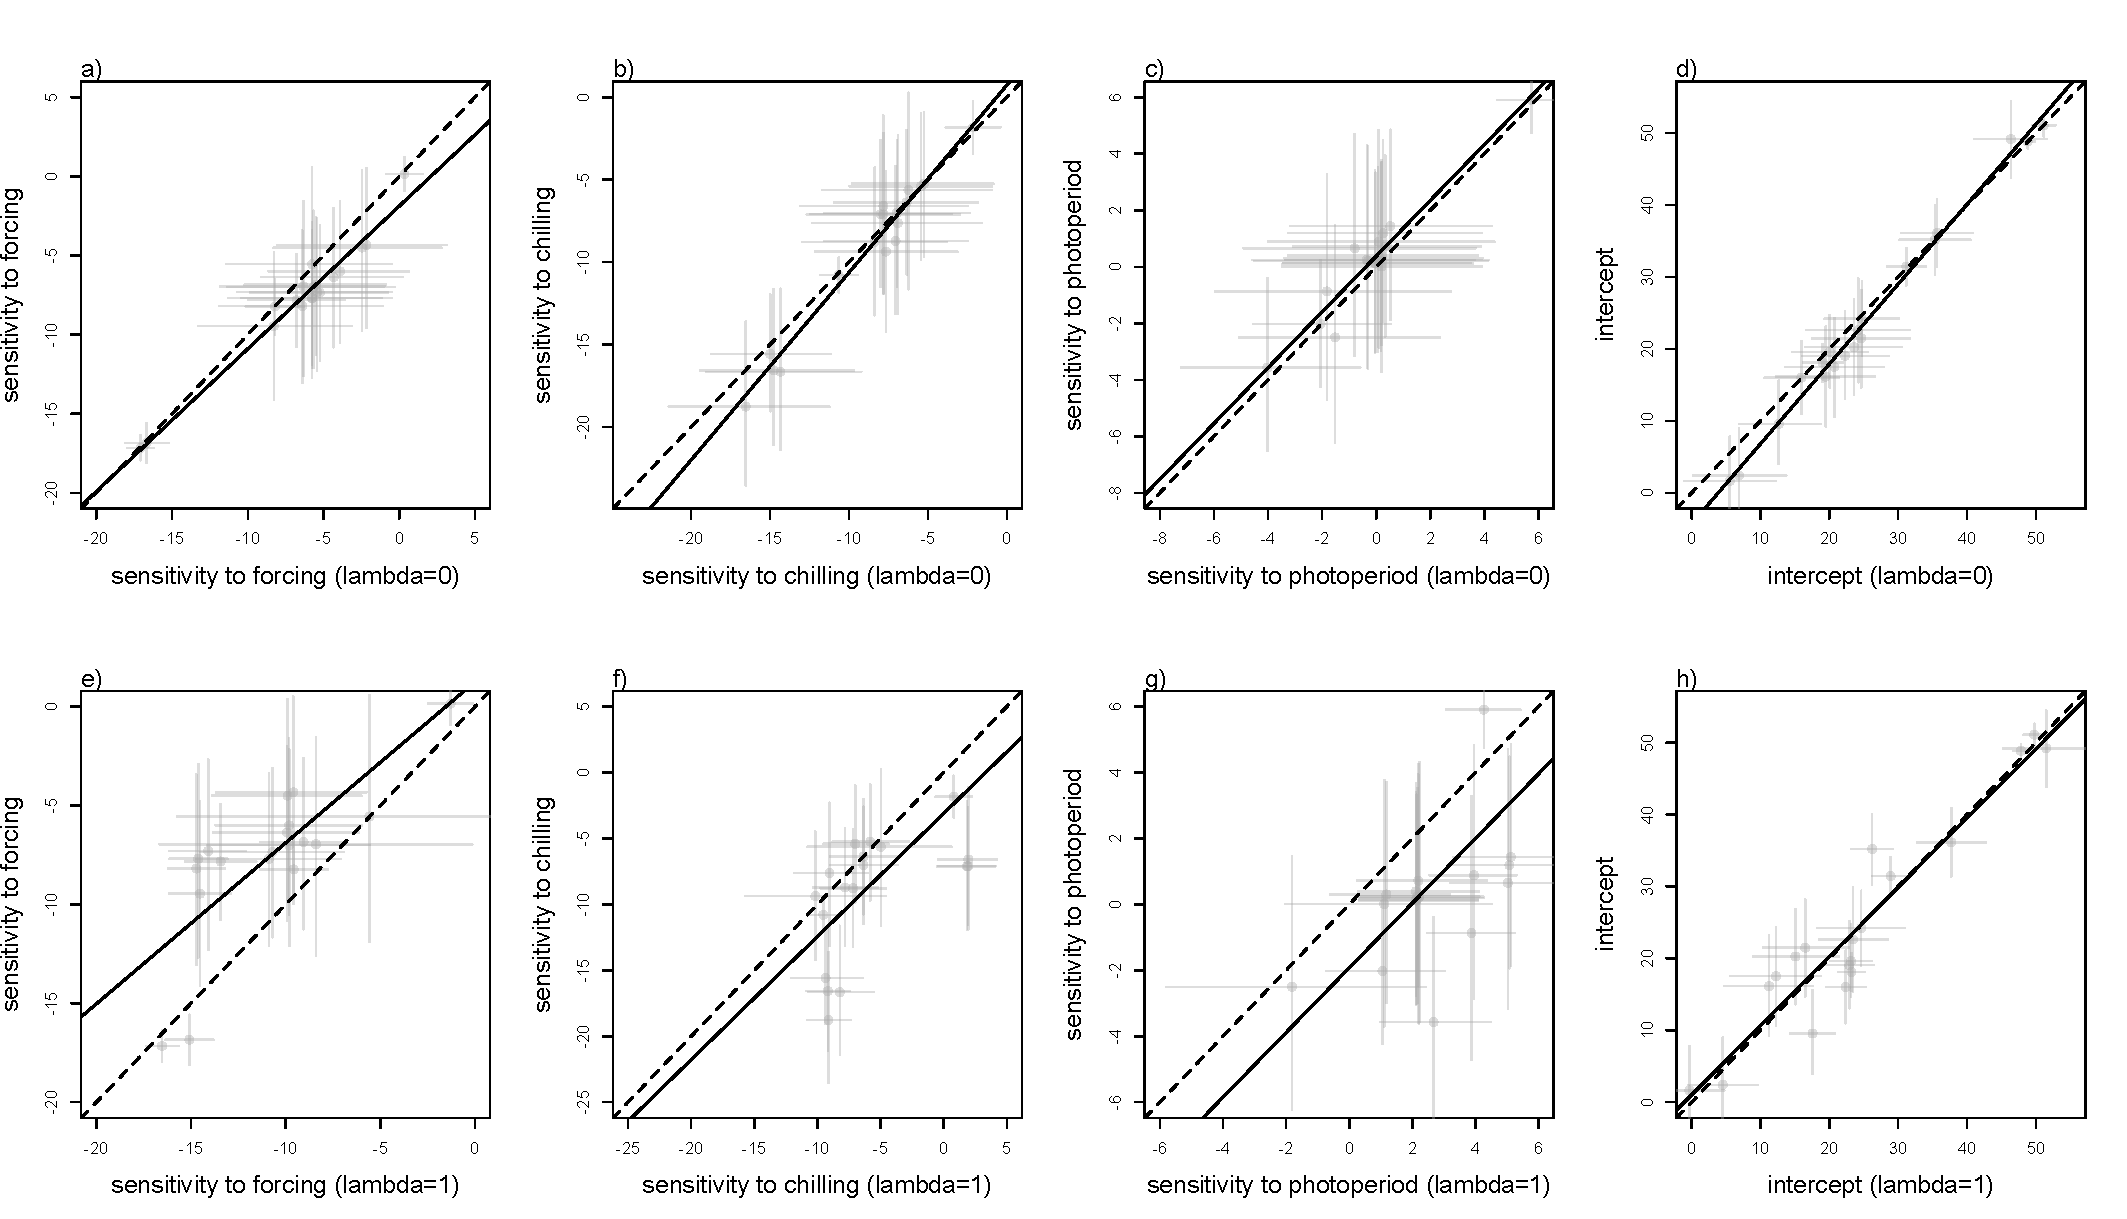
\includegraphics[width=14cm]{../../analyses/phylogeny/figures/Est_correls_vs_lamb01_gymno.pdf}
  \caption{Correlations between model parameters as estimated by the full model and the models where lambda is constrained to be equal zero (upper row) or one (bottom row), for gymnosperms. Panels correspond to sensitivity to forcing (a,e), to chilling (b,f), to photoperiod (c,g) and to model intercepts (d,h).}
  \label{fig:correls_gymno}
  \end{center}
\end{figure}



% IMC Mar21 - I'm guessing we are going to merge some of the tables below. TBD what we keep for the main text and what is sent to a supp.
\begin{table}[H]
\begin{center}
\caption{Full model parameters estimated for 192 angiosperm species.}
\begin{tabular}{@{}lcccccc@{}}
\toprule
\textbf{parameter}             & \multicolumn{1}{l}{\textbf{mean}} & \multicolumn{1}{l}{\textbf{sd}} & \multicolumn{1}{l}{\textbf{2.50\%}} & \multicolumn{1}{l}{\textbf{50\%}} & \multicolumn{1}{l}{\textbf{97.50\%}} & \multicolumn{1}{l}{\textbf{n\_eff}} \\ \midrule
$\mu_\alpha$                   & 30.57                             & 3.41                            & 23.68                               & 30.59                             & 37.14                                & 5031.19                             \\
$\mu_\beta_{forcing}$          & -5.84                             & 2.01                            & -9.72                               & -5.89                             & -1.79                                & 2374.73                             \\
$\mu_\beta_{chilling}$         & -7.19                             & 2.03                            & -11.15                              & -7.18                             & -3.18                                & 3694.93                             \\
$\mu_\beta_{photoperiod}$      & -1.37                             & 0.76                            & -2.92                               & -1.35                             & 0.14                                 & 1565.41                             \\
$\lambda_\alpha$               & 0.35                              & 0.10                            & 0.16                                & 0.34                              & 0.56                                 & 3416.51                             \\
$\lambda_\beta_{forcing}$      & 0.68                              & 0.20                            & 0.23                                & 0.71                              & 0.98                                 & 185.35                              \\
$\lambda_\beta_{chilling}$     & 0.56                              & 0.15                            & 0.25                                & 0.56                              & 0.83                                 & 738.57                              \\
$\lambda_\beta_{photoperiod}$  & 0.36                              & 0.24                            & 0.02                                & 0.33                              & 0.88                                 & 296.51                              \\
$\sigma_\alpha^2$              & 15.93                             & 1.17                            & 13.84                               & 15.85                             & 18.41                                & 2988.37                             \\
$\sigma_\beta^2_{forcing}$     & 5.84                              & 1.04                            & 4.03                                & 5.78                              & 8.15                                 & 502.74                              \\
$\sigma_\beta^2_{chilling}$    & 7.05                              & 0.87                            & 5.48                                & 7.02                              & 8.92                                 & 1026.77                             \\
$\sigma_\beta^2_{photoperiod}$ & 2.45                              & 0.41                            & 1.74                                & 2.42                              & 3.32                                 & 469.46                              \\
$\sigma_y^2$                   & 12.81                             & 0.18                            & 12.47                               & 12.80                             & 13.17                                & 4017.16                             \\ \bottomrule
\end{tabular}
\end{center}
\label{tab:modelanglamb}
\end{table}


\begin{table}[H]
 \begin{center}
\caption{Full model parameters estimated for 19 gymnosperm species.}
\begin{tabular}{@{}lcccccc@{}}
\toprule
\textbf{parameter}             & \multicolumn{1}{l}{\textbf{mean}} & \multicolumn{1}{l}{\textbf{sd}} & \multicolumn{1}{l}{\textbf{2.50\%}} & \multicolumn{1}{l}{\textbf{50\%}} & \multicolumn{1}{l}{\textbf{97.50\%}} & \multicolumn{1}{l}{\textbf{n\_eff}} \\ \midrule
$\mu_\alpha$                   & 25.75                             & 4.50                            & 16.88                               & 25.73                             & 34.73                                & 33151.86                            \\
$\mu_\beta_{forcing}$          & -5.92                             & 3.80                            & -12.97                              & -6.05                             & 1.90                                 & 16443.03                            \\
$\mu_\beta_{chilling}$         & -8.11                             & 3.63                            & -15.31                              & -8.09                             & -0.94                                & 21379.81                            \\
$\mu_\beta_{photoperiod}$      & -0.88                             & 3.33                            & -8.01                               & -0.67                             & 5.19                                 & 16301.93                            \\
$\lambda_\alpha$               & 0.47                              & 0.26                            & 0.02                                & 0.48                              & 0.90                                 & 15934.03                            \\
$\lambda_\beta_{forcing}$      & 0.36                              & 0.23                            & 0.02                                & 0.33                              & 0.84                                 & 14336.60                            \\
$\lambda_\beta_{chilling}$     & 0.32                              & 0.23                            & 0.01                                & 0.28                              & 0.82                                 & 13230.88                            \\
$\lambda_\beta_{photoperiod}$  & 0.37                              & 0.24                            & 0.02                                & 0.34                              & 0.88                                 & 11199.49                            \\
$\sigma_\alpha^2$              & 23.47                             & 6.20                            & 13.87                               & 22.59                             & 37.81                                & 18272.58                            \\
$\sigma_\beta^2_{forcing}$     & 8.89                              & 2.45                            & 4.96                                & 8.60                              & 14.51                                & 8126.51                             \\
$\sigma_\beta^2_{chilling}$    & 10.47                             & 2.66                            & 5.78                                & 10.30                             & 16.17                                & 8539.38                             \\
$\sigma_\beta^2_{photoperiod}$ & 7.18                              & 2.29                            & 3.29                                & 6.96                              & 12.25                                & 5625.69                             \\
$\sigma_y^2$                   & 15.81                             & 0.41                            & 15.04                               & 15.81                             & 16.63                                & 28640.16                            \\ \bottomrule
\end{tabular}
\end{center}
\label{tab:modelgymlamb}
\end{table}





\pagebreak
%\bibliographystyle{refs/bibstyles/amnat.bst}% 
%\bibliography{refs/phylorefs.bib}



\end{document}